\section{Ordinary Least Squares}
This section will introduce the method of ordinary least squares for estimating parameters in a linear regression model.

\subsection{Least Squares}
The main idea behind the least squares is to minimize the sum of squared residuals, also known as SSR. 
Given a set of data points in the plane how might one find the line that best fit the data, one way is to choose the line that minimizes the sum of squared residuals.
In figure \ref{fig:example_simple_linear_regression} an example of a simple linear regression can be seen. 
The figure illustrates the log price plotted against the age of property sold by Home in Aalborg within the year 2012.
\begin{figure}[h]
    \centering
    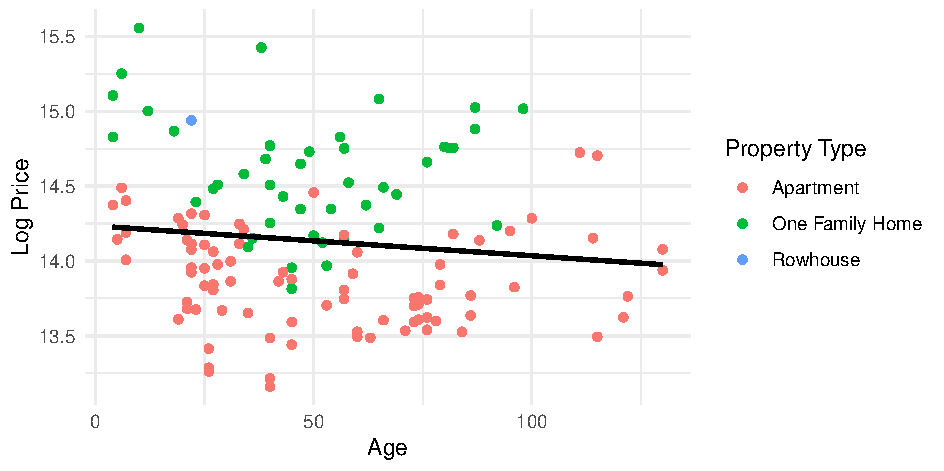
\includegraphics[width = 0.9\textwidth]{figures/Ordinary_Least_Squares/example_linear_regression.pdf}
    \caption{Age and log price of property sold in 2012 by Home in Aalborg.}
    \label{fig:example_simple_linear_regression}
\end{figure}

The dataset has observations of the form $\{a_i, log(p_i)\}$ with $i = 1, \ldots, 130$. The age of property is seen as the independent variable and the log price as the dependent variable.
We can assume, albeit naive considering figure \ref{fig:example_simple_linear_regression}, that there is a linear relationship between age and log price of the property in question.
This can be formulated as
\begin{align}\label{eq:approx_linear_relationship}
    \log(p) \approx \beta_0 + \beta_1 a
\end{align}
where $log(p)$ and $a$ denotes the log price and age respectively.
The right side \eqref{eq:approx_linear_relationship} is the model function in our case.
The function is on the form $f(a, \boldsymbol{\beta})$, where $\boldsymbol{\beta}$ is a $2 \times 1$ vector containing the parameters $\beta_0$ and $\beta_1$.
The goal is now to find $\boldsymbol{\beta}$ that minimizes the sum of squared residuals.
For the $i$'th observation the residual is defined as $r_i = log(p_i) - f(a, \boldsymbol{\beta})$.
With the notation in place we can now write the sum of squared residuals as
\begin{align}\label{eq:SSR}
  \ssr(\boldsymbol{\beta}) = \sum_{i = 1}^{130} r_i^2 = \sum_{i = 1}^{130} \left( log(p_i) - f(a, \boldsymbol{\beta}) \right)^2
\end{align}

\subsection{Parameter Estimation in Matrix Form}
Estimating parameters for a multiple linear regression model in matrix form still translates to minimizing the sum of squared residuals.
The sum of squared residuals now take the form
\begin{align*}
    \ssr(\mathbf{b}) = \nsum (y_i - \mathbf{x}_i\mathbf{b})^2.
\end{align*}
where $y_i$ denotes the price of the property $i$ and $\mathbf{x}_i$ denotes the $i$'th row in the design matrix $\mathbf{x}$.
It is therefore a row vector of the form
\begin{align*}
    \mathbf{x}_i = \begin{bmatrix} 1 & x_{i1} & \cdots & x_{ik} \end{bmatrix}.
\end{align*}
Suppose that $\betahat$ minimizes the sum of squared residuals, that is
\begin{align*}
    \betahat = \underset{\mathbf{b}}{\argmin} \nsum (y_i - \mathbf{x}_i\mathbf{b})^2.
\end{align*}
Then $\betahat$ must satisfy the condition $\nabla \ssr(\betahat) = 0$.
Taking the derivative w.r.t. $\mathbf{b}$ yields
\begin{align}\label{eq:ssr_derivative}
    \frac{\partial \ssr(\mathbf{b})}{\partial \mathbf{b}} 
    =  \nsum -2(y_i - \mathbf{x}_i \mathbf{b})\mathbf{x}_i
\end{align}
The expression $\nabla \ssr (\betahat) = 0$ can now be rewritten as
\begin{align*}
    \nsum -2(y_i - \mathbf{x}_i \betahat)\mathbf{x}_i = 0 
    \quad \Rightarrow \quad
    \nsum \mathbf{x}_i^\top(y_i - \mathbf{x}_i \betahat) = 0
\end{align*}
by taking the transpose and dividing by two.
The condition is now a vector of size $(k + 1) \times 1$ and thus represents a system of $k + 1$ equations with $k + 1$ unknowns.
Writing the vector as a system of equations gives the following $k + 1$ equations
\begin{align}\label{eq:multiple_linear_regression_equations}
\begin{split}
    \nsum (y_i - \betahat_0 -  \mathbf{x}_{i1} \betahat_1 - \ldots - \betahat_k \mathbf{x}_{ik}) &= 0 \\
    \nsum \mathbf{x}_{i1}(y_i - \betahat_0 -  \mathbf{x}_{i1} \betahat_1 - \ldots - \betahat_k \mathbf{x}_{ik}) &= 0 \\
    &\vdots \\
    \nsum \mathbf{x}_{ik}(y_i - \betahat_0 -  \mathbf{x}_{i1} \betahat_1 - \ldots - \betahat_k \mathbf{x}_{ik}) &= 0
\end{split}
\end{align}
Returning to the notation used in \eqref{eq:multiple_linear_regression_model}, \eqref{eq:multiple_linear_regression_equations} will now be rewritten to matrix notation
\begin{align}
    \mathbf{X}^\top(\mathbf{y} - \mathbf{X}\betahat) &= \mathbf{0} \nonumber\\
    \mathbf{X}^\top\mathbf{y} - \mathbf{X}^\top\mathbf{X}\betahat &= \mathbf{0}\nonumber\\
    \mathbf{X}^\top\mathbf{X}\betahat &= \mathbf{X}^\top\mathbf{y}\label{eq:equation_from} \\
    \betahat &= \left(\mathbf{X}^\top\mathbf{X}\right)^{-1}\mathbf{X}^\top\mathbf{y}.\label{eq:equation_to}
\end{align}
Going from \eqref{eq:equation_from} to \eqref{eq:equation_to} one must assume that $\mathbf{X}^\top\mathbf{X}$ is non-singular and thereby invertible.
It turns out that this is not the only assumption we have to make, there are in fact five assumptions related to the OLS estimator.
These assumptions will now be listed.
\begin{assumption}[Linear in parameters]
    The model can be written as $\mathbf{y} = \mathbf{X}\boldsymbol{\beta} + \boldsymbol{\varepsilon}$ where $\mathbf{y}$ is an observed $n \times 1$ vector, $\mathbf{X}$ is an $n \times (k + 1)$ observed matrix, and $\boldsymbol{\varepsilon}$ is an $n \times 1$ vector of unobserved errors or disturbances \cite[p. 1]{Wooldridge2012}.
\end{assumption}
\begin{assumption}[No perfect collinearity]
    The matrix $\mathbf{X}$ has rank $(k + 1)$.
\end{assumption}
\begin{assumption}[Zero conditional mean]
    Conditional on the entire matrix $\mathbf{X}$, each error $\varepsilon_i$ has zero mean, i.e.
    \begin{align*}
        E(\varepsilon_i | \mathbf{X}) = 0, \quad i = 1, 2, \ldots, n.
    \end{align*}
\end{assumption}
\begin{assumption}[Homoskedasticity and no serial correlation]
    This assumptions have to two parts, the first part, regarding \homo states that
    \begin{align*}
        \var(\varepsilon | \mathbf{X}) = \sigma^2, \quad i = 1,2, \ldots, n.
    \end{align*}
    The second part, regarding serial corellation, states that
    \begin{align*}
        \cov(\varepsilon_i, \varepsilon_j | \mathbf{X}) = 0, \quad \text{for all} \ i \neq j.
    \end{align*}
    In matrix form these to assumptions together becomes
    \begin{align*}
        \var(\boldsymbol{\varepsilon} | \mathbf{X}) = \sigma^2\mathbf{I}_{n\times n}.
    \end{align*}
\end{assumption}
\begin{assumption}[Normality of errors]
    Conditional on $\mathbf{X}$, the $\varepsilon_i$ are independent and identically distributed as $N(0, \sigma^2)$. Equivalently, $\boldsymbol{\varepsilon}$ given $\mathbf{X}$ is distributed as multivariate normal with mean zero and variance-covariance matrix $\sigma^2 \mathbf{I}_{n \times n}$, i.e. $\boldsymbol{\varepsilon} \sim N(\mathbf{0}, \sigma^2 \mathbf{I}_{n \times n})$.
\end{assumption}